\subsection{هندسی}
الگوریتم هندسی \lr{A* } نخستین بار در مسائل مسیریابی در محیط‌های بندری بیان شد ؛ در این محیط ها عامل علاوه بروظیفه ی حمل و نقل کالا، بایستی خود را در زمان منناسب به ایستگاه شارژ می رساندند . این الگوریتم اساساً برای رسیدگی به مسائلی مانند زوایای چرخش بزرگ، گره‌های متعددی که معمولاً در مسیرهای متقاطع وجود دارند و مسیرهای دندان اره‌ای که توسط الگوریتم کلاسیک  \lr{A* } تولید می‌شوند ، توسعه داده شد.  
\par
\lr{A* } هندسی ابتدا یک نقشه شبکه ای از محیط ایجاد می کند و موانع غیر ضروری را از بین می برد و اشکال نامنظم را منظم می کند. پس از این، الگوریتم کلاسیک  \lr{A* } برای به دست آوردن یک مسیر بدون مانع از موقعیت شروع تا موقعیت نهایی اعمال می شود. چنین مسیرهایی به عنوان لیستی از نقاط به دست می آیند. سپس الگوریتم هندسی  \lr{A* } با استفاده از توابع فیلتر
\lr{P(x, y)} 
(\ref{crosspath:fig1})
و
\lr{W(x, y)}
شکل 
(\ref{sawtooth:fig2})
گره های نامعتبر را از این لیست فیلتر می کند. نتایج حاصل از کار این فیلتر نشان می دهد که تعداد گره های بررسی شدده ی حاصل از این ورژن نسبت به حالت کلاسیک کاهش قابل ملاحظه ای یافته است و در یک نمونه مسئله از 2246 به 109 مورد رسیده است . در 
\ref{a_star}
و
\ref{geo}
نقاط آبی گره های بررسی شده توسط الگوریتم و نقاط قرمز مسینهایی الگوریتم می باشند .

\begin{figure}[h]
	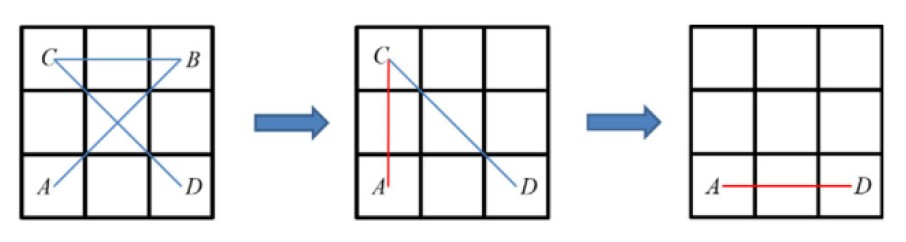
\includegraphics[scale=0.6]{cross_filter}
	\centering
	\caption{بهینه سازی  مسیر با استفاده از فیلتر \lr{P(x,y)}}
	\cite{paliwal2023survey}
	\label{crosspath:fig1}
\end{figure} 

\begin{figure}[h]
	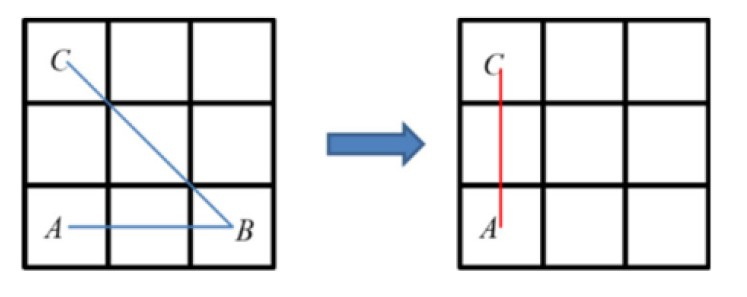
\includegraphics[scale=0.6]{sawtooth}
	\centering
	\caption{بهینه سازی  مسیر با استفاده از فیلتر \lr{W(x,y)}}
	\cite{paliwal2023survey}
	\label{sawtooth:fig2}
\end{figure}
\begin{figure}[h]
	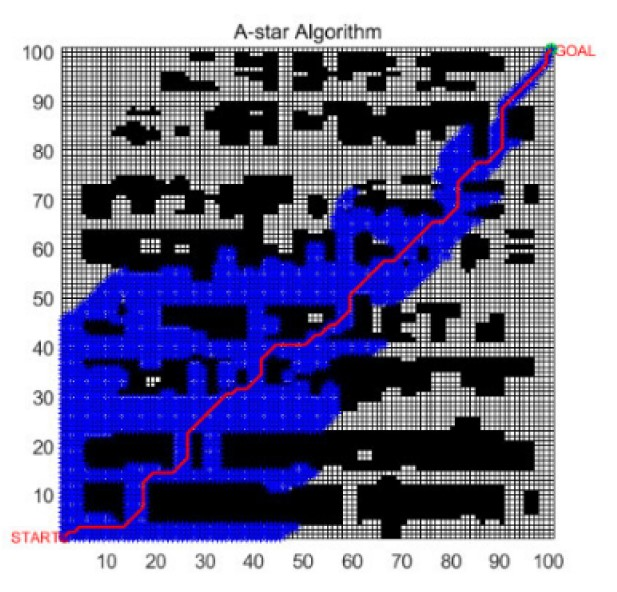
\includegraphics[scale=0.7]{a_star_vs_geo}
	\centering
	\caption{مسیر یابی توسط الگوریتم کلاسیک \lr{A*}}
	\cite{paliwal2023survey}
	\label{a_star}
\end{figure}

\begin{figure}[h]
	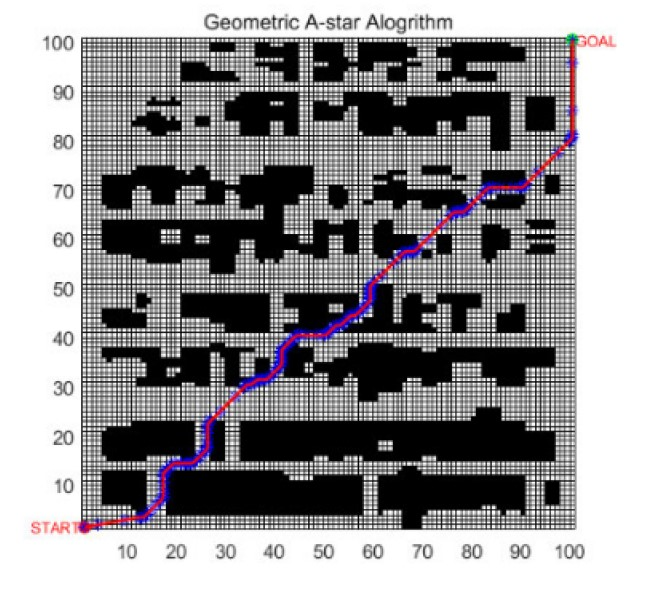
\includegraphics[scale=0.7]{geo}
	\centering
	\caption{ مسیر یابی توسط الگوریتم روش هندسی \lr{A*}}
	\cite{paliwal2023survey}
	\label{geo}
\end{figure}